% Sopra-Steria, Scotland, UK

%\subsubsection{The Smart Patient Health Record}

%\noindent 
%% VJ: Maybe put some of this above
%The Smart Patient Health Record (SPHR) is the combination of a patient's data, and the patient's control over access to their data. By gathering together all of the data into a single source, we allow the patient to have direct control over who can see what. 

%Further more, if the patient is treated outside of their home treatment centre, the patient will be able to share important information with this new treatment centre digitally. Any treatments they receive at this new treatment centre will also be recorded into the SPHR.


%% VJ: We should put this somewhere in the background
%\subsubsection{Data Vault}

%Our choice for database format is Data Vault. This is a highly flexible format that will allow for continuous changes to what is stored in them, future-proofing the underlying design of the SPHR.

%The main difference between a Data Vault and a traditional style of database is the way the data is organised, with features being grouped by core concept as opposed to their a general theme. In Data Vaults these elements are called Hubs. Hubs are joined together via many-to-many relationships called Links, with the features themselves being grouped in Satellites.

%For Serums we have chosen the core concepts of Time, Person, Object, Location, and Event (TPOLE) for our Hubs. These five concepts will cover every aspect of patient-doctor-treatment interaction.
\begin{figure}
    \centering
    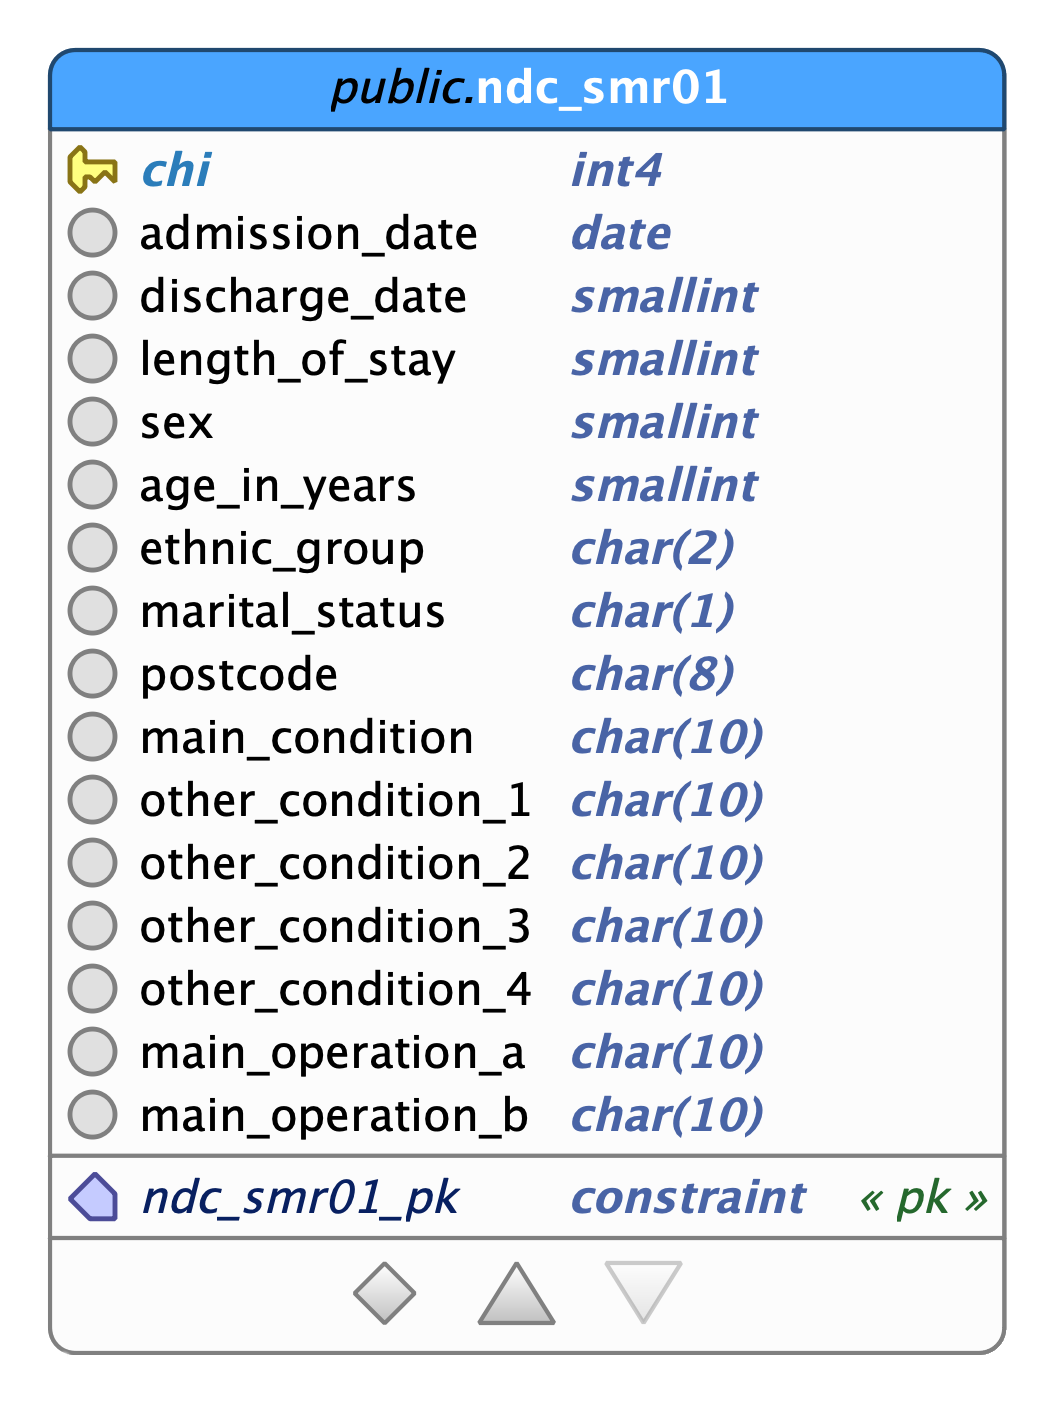
\includegraphics[width=45mm]{images/DataVault/smr01_source.png}
    \caption{Example of source table}
    \label{fig:smr01_source}
\end{figure}

\begin{figure}
    \centering
    \includegraphics[width=80mm]{images/DataVault/DataVault.pdf}
    \caption{Example of source table abstracted into Data Vault}
    \label{fig:dv_smr01}
\end{figure}

For example, Figure~\ref{fig:smr01_source} shows a part of the Edinburgh Cancer Gateway Centre use case, described in more detail in Section~\ref{sec:XX}. It contains information about one hospital visit of one patient. When abstracted into a data vault, the person hub would refer to patients, the time hub would refer to the dates and times of the hospital visits, and the object hub would contain the operations. The person hub contains the \emph{person demographic details} satellite, the time hub contains the \emph{admission date} satellite and the object hub contains the \emph{operations} and \emph{conditions} satellites (See Figure~\ref{fig:dv_smr01}). 



%\begin{figure}[H]
 %   \centering
  %  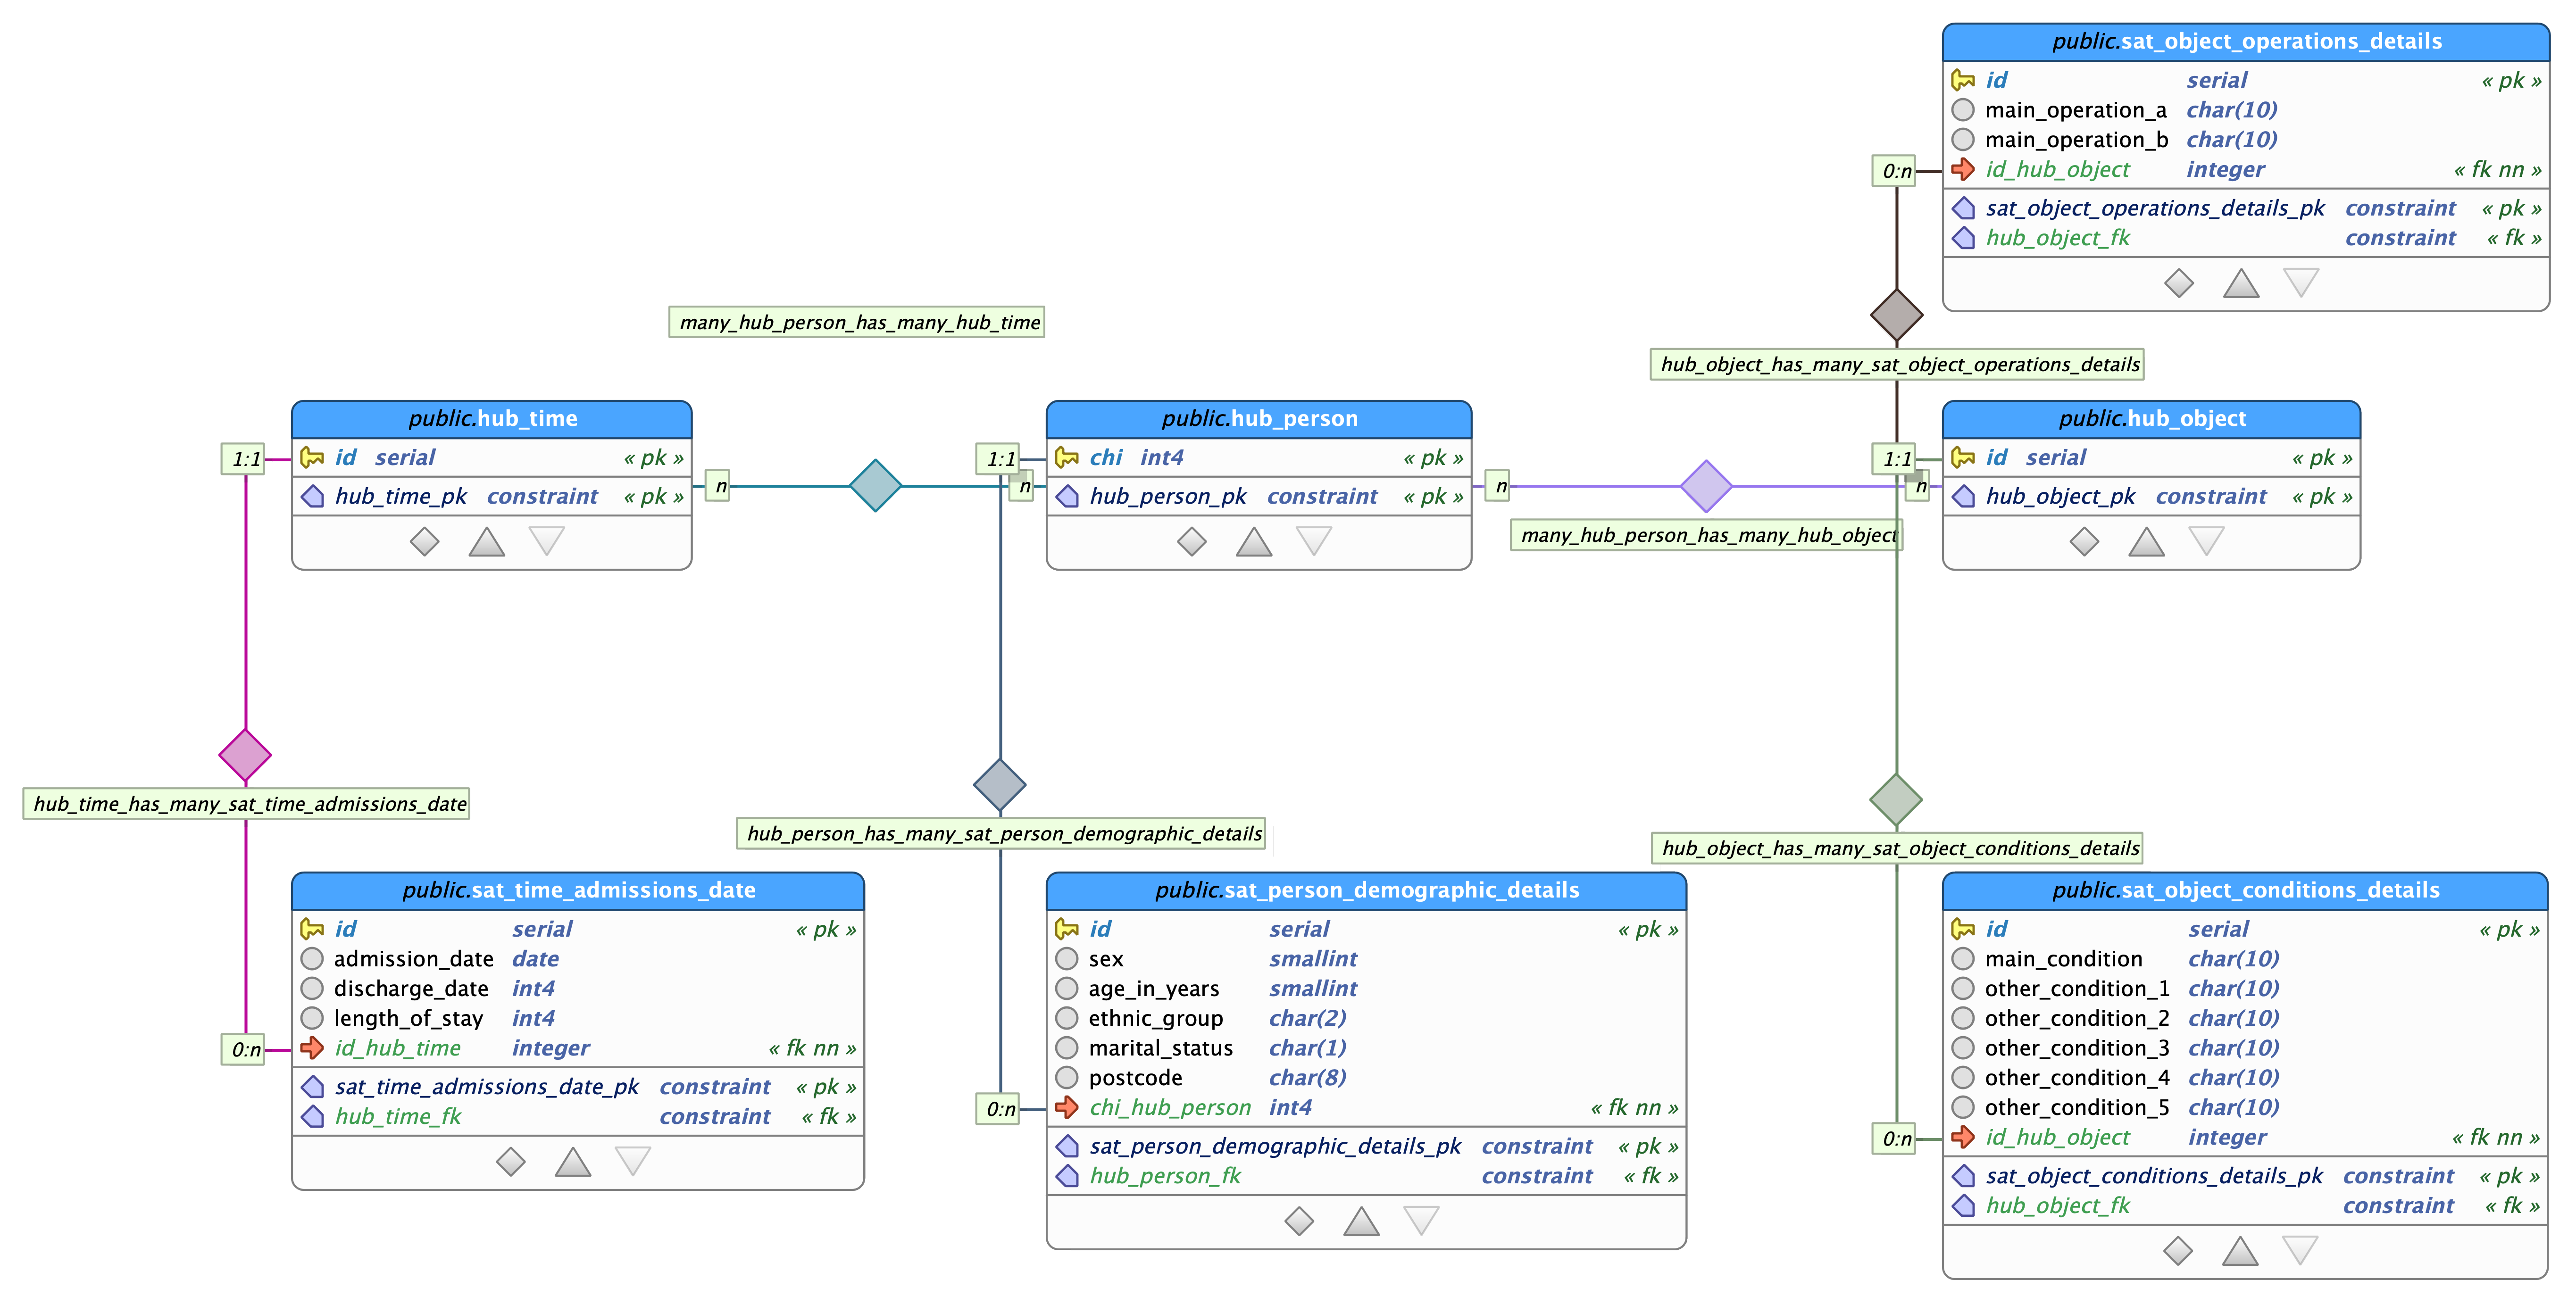
\includegraphics[width=70mm]{images/DataVault/dv_ndc_smr01_db.png}
   % \caption{Example of source table abstracted into Data Vault}
    %\label{fig:dv_smr01}
%\end{figure}

%Note that not all of the TPOLE hubs have been generated in this abstraction. As more sources are added the SPHR would fill out with these hubs as well as many more satellites:

%\begin{figure}[H]
%    \centering
 %   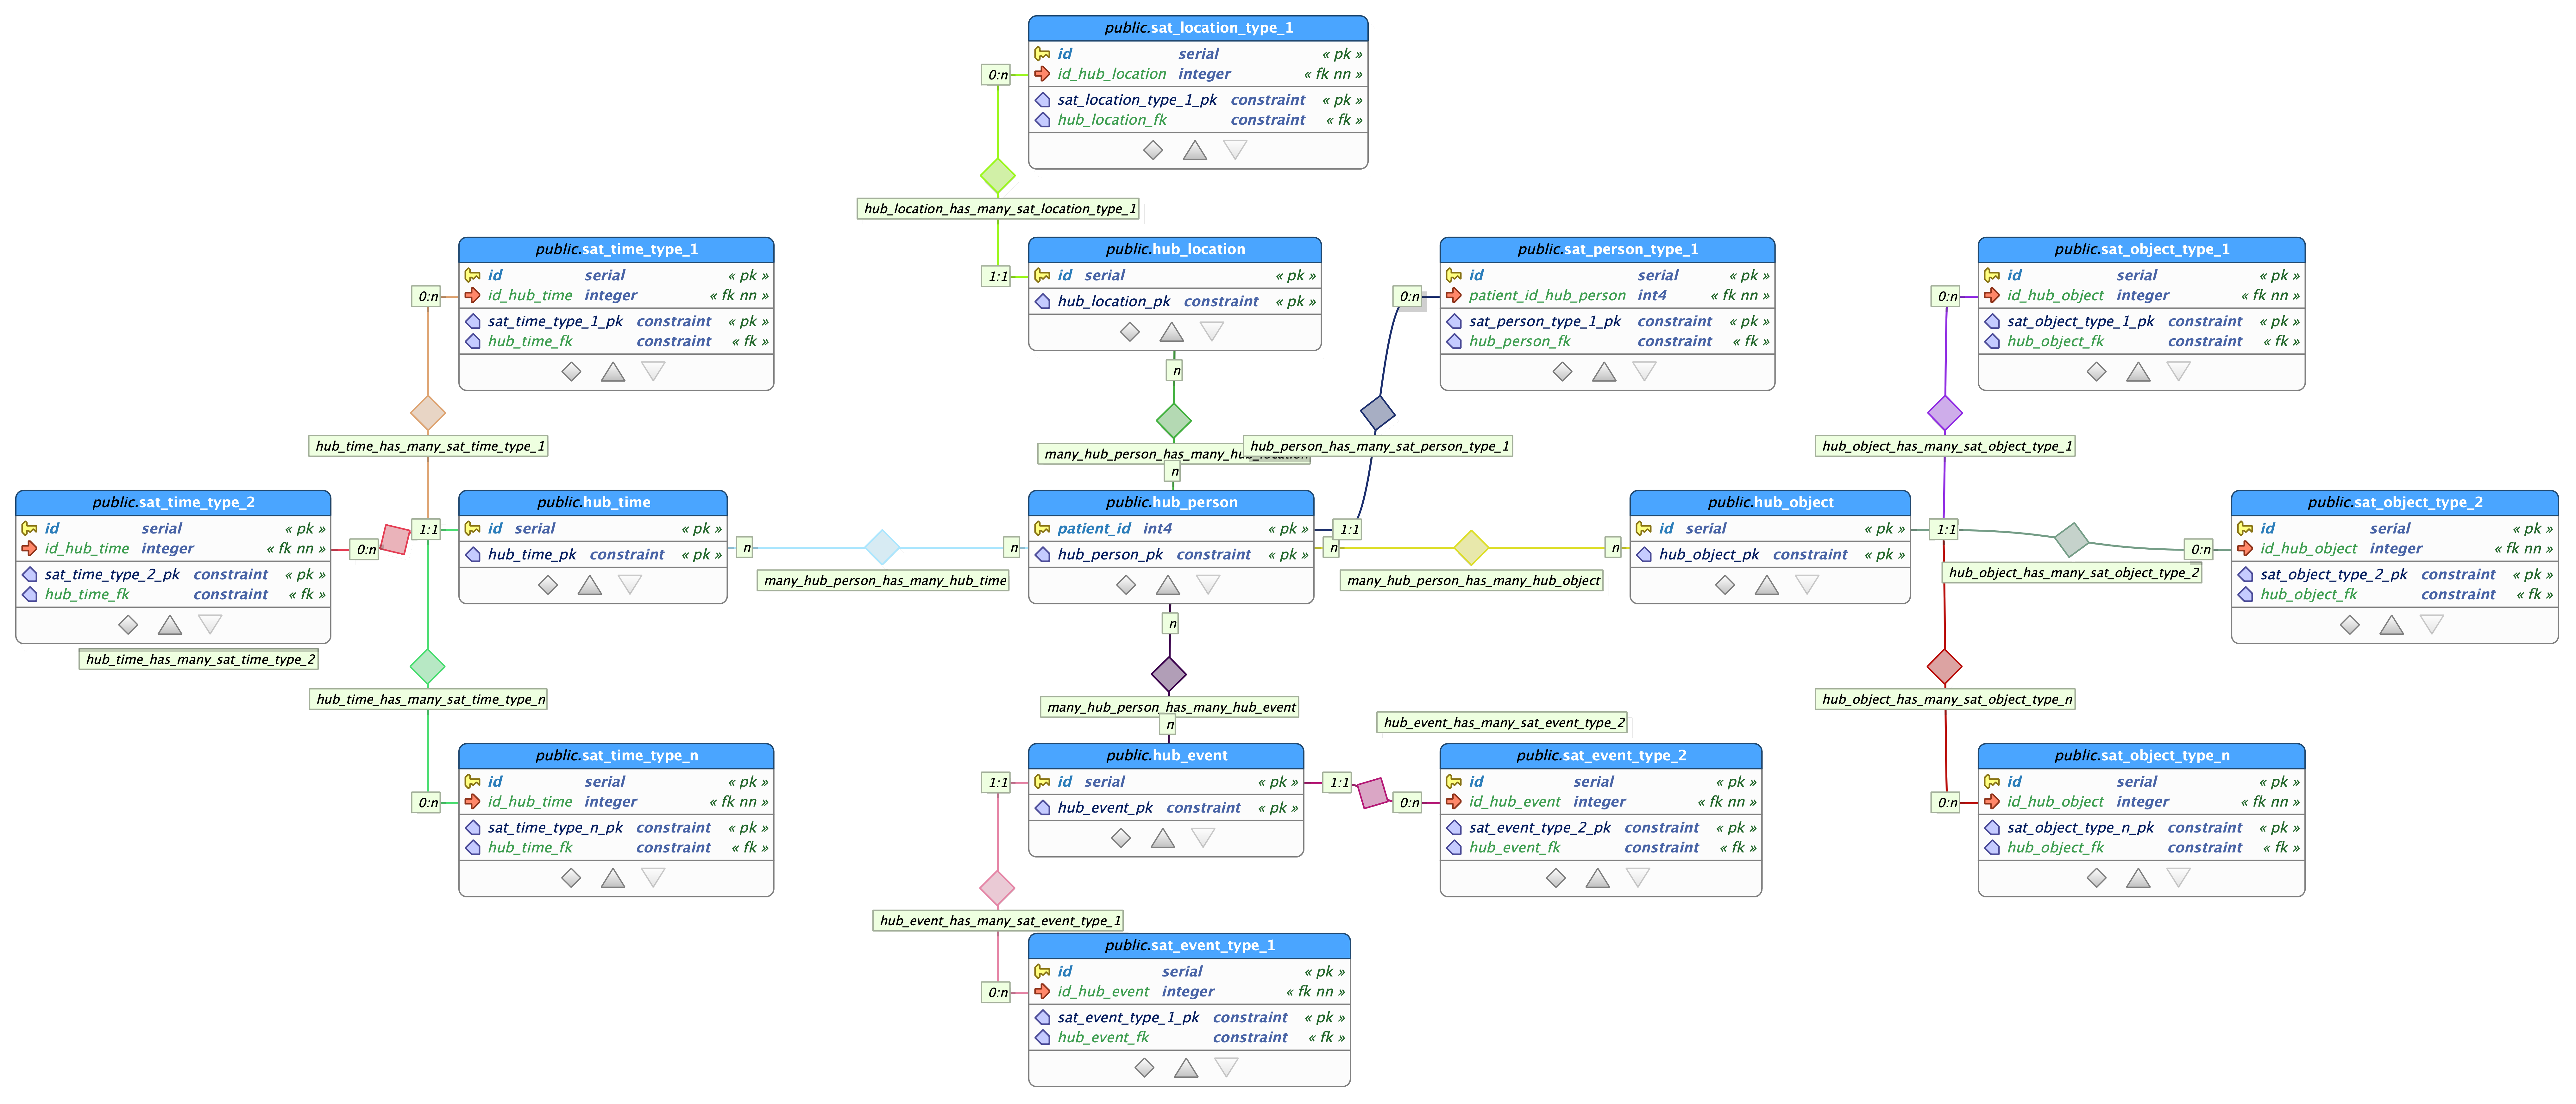
\includegraphics[width=70mm]{images/DataVault/universal_smart_patient_record.png}
  %  \caption{Example of an expanded Data Vault}
   % \label{fig:dv_expanded}
%\end{figure}
